% -----------------------------
% 大作业 —— 模板
% 作者:<你的姓名>
% 日期:<YYYY-MM-DD>
% -----------------------------
\documentclass[11pt,a4paper]{article}
\usepackage{ctex}
% ======= 基本宏包 =======

\usepackage[utf8]{inputenc}

% ======= 代码高亮(可选) =======
\usepackage{listings}
\lstset{
  inputencoding=utf8,
  extendedchars=true,
  basicstyle=\ttfamily\small,
  keywordstyle=\color{blue},
  commentstyle=\color{gray},
  numbers=left,
  numberstyle=\tiny,
  breaklines=true,
  frame=single
}

\usepackage[T1]{fontenc}
\usepackage{geometry}
\geometry{margin=2.5cm}
\usepackage{amsmath, amsfonts, amssymb}
\usepackage{graphicx}
\usepackage{booktabs}
\usepackage{hyperref}
\usepackage{caption}
\usepackage{float}
\usepackage{xcolor}
\usepackage{longtable}
\usepackage{siunitx}


% ======= 文章信息 =======
\title{\textbf{人民币汇率时间序列建模与预测分析}}
\author{<计科33 胡加怿>\\<2023011431>\\<hu-jy23@mails.tsinghua.edu.cn>}
% \date{<2025.5.7>}

\begin{document}
\maketitle

% ---------------------------
% 自动生成目录
% ---------------------------
\tableofcontents
\newpage

% ---------------------------
% 研究背景与问题提出
% ---------------------------
\section{研究背景与问题提出}
简要说明汇率对宏观经济与国际贸易的重要性,并指出人民币汇率近年来呈现出明显的结构性变化与波动性特征。本研究以 2000--2025 年的 USD/CNY 日度和月度汇率为对象,围绕以下问题开展时间序列建模:

\begin{itemize}
  \item 汇率序列是否平稳?是否存在单位根与结构突变?
  \item ARIMA 与 SARIMA 模型谁更适合用于汇率预测?
  \item 是否存在周期性成分(如年度效应)?若有应如何建模?
\end{itemize}

% ---------------------------
% 数据来源与预处理
% ---------------------------
\section{数据来源与处理}

本研究使用的数据来源于 \href{https://www.investing.com/}{Investing.com} 网站公开的 USD/CNY 日度汇率历史记录,所使用变量为每日收盘汇率(Price),原始数据范围为 1999 年至 2025 年初,具有较高的时间精度与连续性。图~\ref{fig:rate-full} 展示了 1999--2020 年期间的汇率趋势。

\begin{figure}[H]
  \centering
  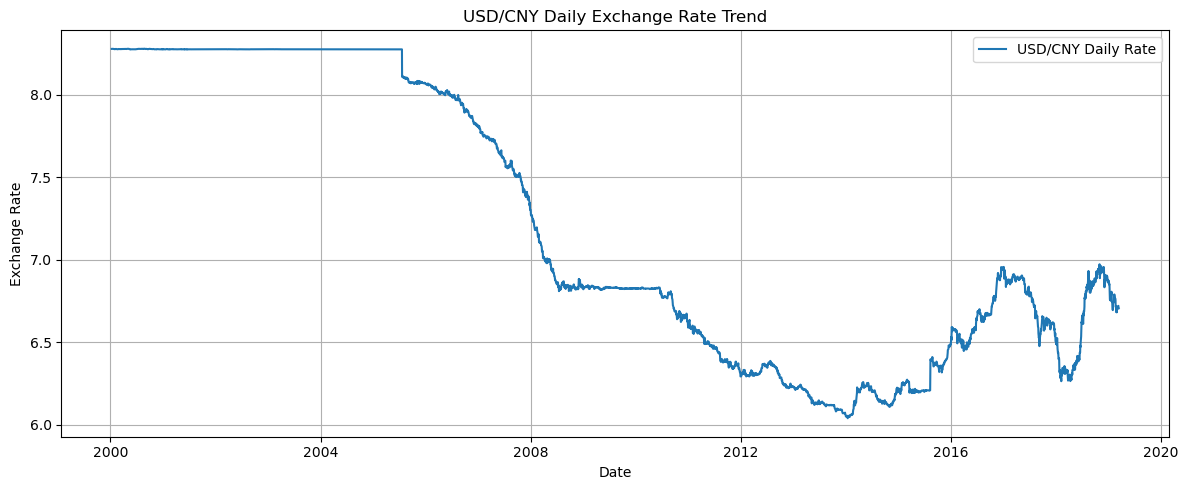
\includegraphics[width=1\textwidth]{./figures/2000-2020.png}
  \caption{USD/CNY 日度汇率走势(1999--2020)}
  \label{fig:rate-full}
\end{figure}

从图中可见,2005 年之前人民币汇率长期固定在 8.27 左右,呈现典型的单一汇率制度特征;2005 年汇改之后开始呈现缓慢升值趋势,并在 2008--2010 年再次短期钉住。由于这段时期政策干预强、波动性极低,不利于开展基于统计特性的模型拟合。

考虑到:
\begin{itemize}
  \item 自 2014 年起,中国汇率制度逐步市场化,汇率波动性明显增强;
  \item 数据完整性与宏观背景(如“8·11”汇改、美联储加息周期、疫情冲击等)更契合结构突变与季节性建模;
  \item 近十年更贴近现实政策关注,便于解释与预测;
\end{itemize}
本文最终选取 2014 年 1 月至 2025 年 5 月的日度数据作为分析窗口,图~\ref{fig:rate-zoom} 展示了这一期间汇率走势的局部放大图。

\begin{figure}[H]
  \centering
  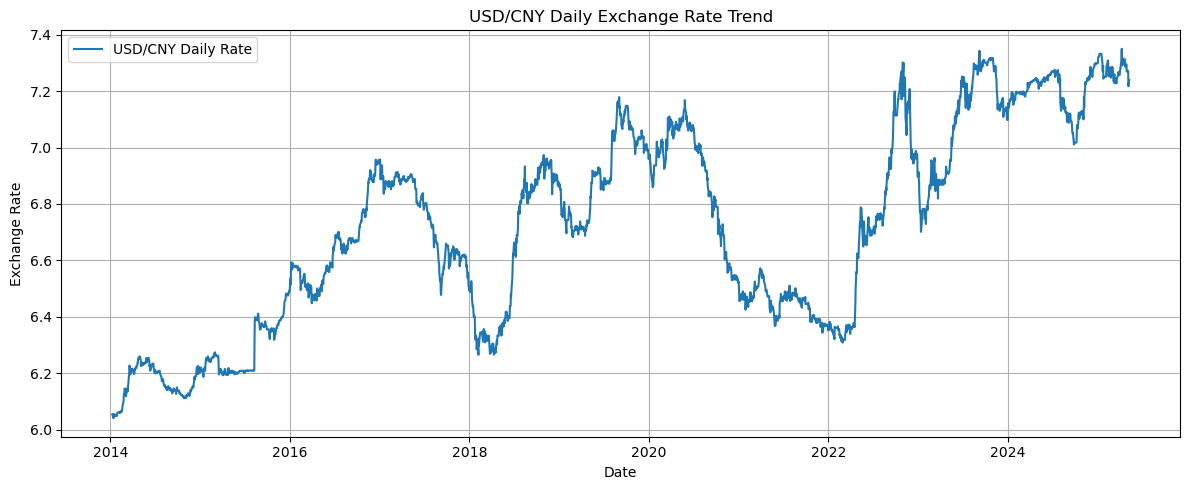
\includegraphics[width=1\textwidth]{./figures/2014-2025.png}
  \caption{USD/CNY 日度汇率走势(2014--2025)}
  \label{fig:rate-zoom}
\end{figure}

\subsection{数据清洗与变换}

数据预处理过程包括以下步骤:
\begin{itemize}
  \item 将原始 CSV 文件中的日期字段统一转换为 \texttt{datetime} 类型,并设为索引;
  \item 删除包含缺失值的行(主要是节假日或数据源空缺);
  \item 按月末重采样(resample to month-end),得到月度汇率时间序列,作为后续分析的建模基础。
\end{itemize}


% ---------------------------
\section{平稳性检验与趋势分析}

\subsection{趋势观察与结构突变检测}

图~\ref{fig:monthly-breaks} 显示了 2014--2025 年人民币兑美元(USD/CNY)月末汇率的走势及其结构突变检测结果。使用 PELT 算法(断点惩罚项 $\texttt{pen}=5$)检测出一个显著突变点,位于 2022 年 10 月,恰对应美联储激进加息与人民币阶段性贬值,表明外部金融冲击对汇率趋势产生结构性影响。

\begin{figure}[H]
  \centering
  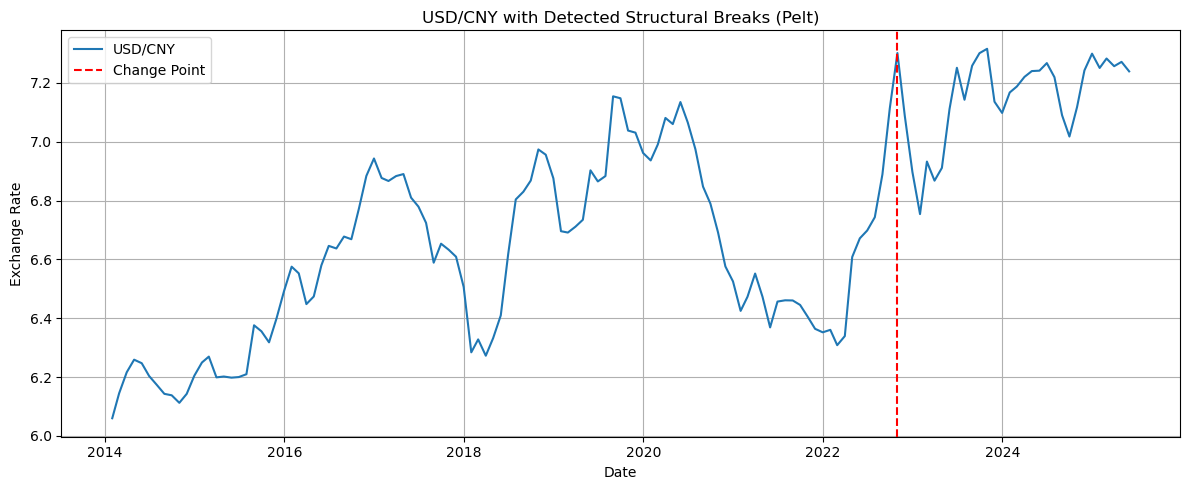
\includegraphics[width=1\textwidth]{./figures/yichang detection.png}
  \caption{USD/CNY 月度汇率与结构突变点(PELT)}
  \label{fig:monthly-breaks}
\end{figure}

\subsection{单位根检验(ADF)与差分平稳性判断}

对原始月度汇率序列进行 ADF 检验,结果如表~\ref{tab:adf-raw} 所示,p 值为 0.2456,未能拒绝单位根假设,说明原序列非平稳。

\vspace{1em}
\begin{table}[H]
  \centering
  \caption{原始月度序列的 ADF 检验结果}
  \begin{tabular}{lccc}
    \toprule
    ADF Statistic & p-value & 1\%临界值 & 5\%临界值 \\
    \midrule
    -2.0973 & 0.2456 & -3.4797 & -2.8832 \\
    \bottomrule
  \end{tabular}
  \label{tab:adf-raw}
\end{table}

为实现平稳性,对序列进行一阶差分,得到差分序列如图~\ref{fig:diff-series} 所示,呈零均值且波动相对稳定的特征。

\begin{figure}[H]
  \centering
  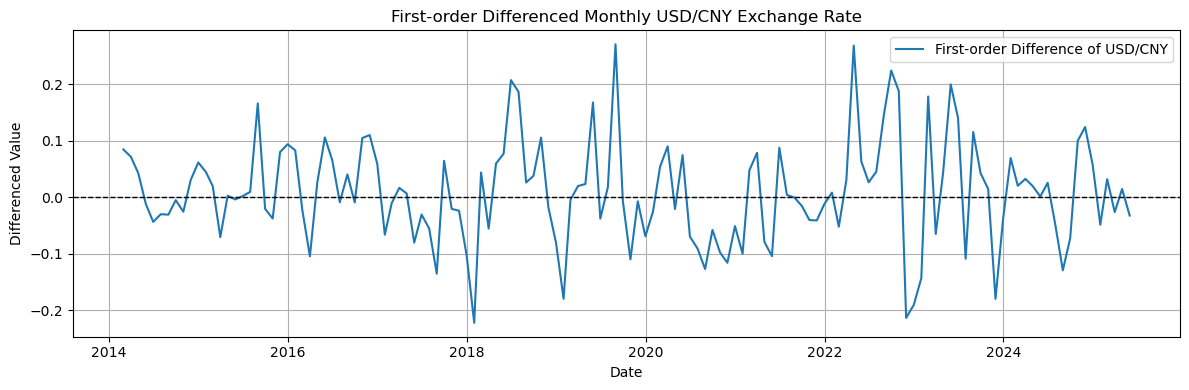
\includegraphics[width=1\textwidth]{./figures/diff1[0].png}
  \caption{USD/CNY 月度汇率一阶差分序列}
  \label{fig:diff-series}
\end{figure}

随后对一阶差分序列进行 ADF 检验(见表~\ref{tab:adf-diff}),p 值接近 0,显著拒绝单位根假设,表明差分后序列为宽平稳。

\begin{table}[H]
  \centering
  \caption{差分序列的 ADF 检验结果}
  \begin{tabular}{lccc}
    \toprule
    ADF Statistic & p-value & 1\%临界值 & 5\%临界值 \\
    \midrule
    -8.0635 & $1.6 \times 10^{-12}$ & -3.4812 & -2.8836 \\
    \bottomrule
  \end{tabular}
  \label{tab:adf-diff}
\end{table}

\subsection{自相关结构分析与季节性探索}

图~\ref{fig:acf-pacf} 展示了一阶差分序列的 ACF 与 PACF 图。其中 ACF 在一阶滞后后快速衰减,PACF 仅在一阶滞后处显著,提示适合采用 ARIMA(0,1,1) 或 ARIMA(1,1,0) 模型。

\begin{figure}[H]
  \centering
  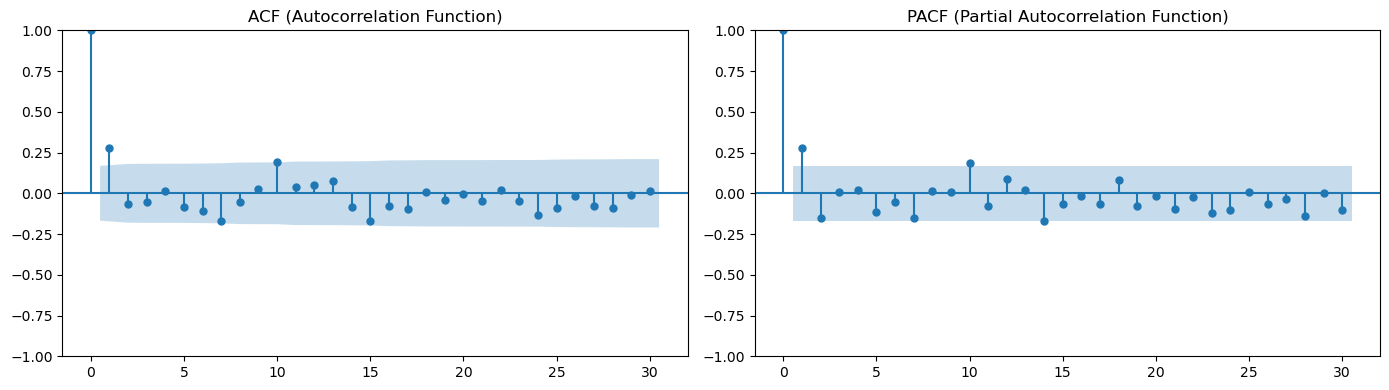
\includegraphics[width=1\textwidth]{./figures/ACF&PACF on diff1[0].png}
  \caption{一阶差分序列的 ACF 与 PACF 图}
  \label{fig:acf-pacf}
\end{figure}

为进一步判断是否存在年度季节性结构,对月度序列进行 12 阶差分,并绘制其 ACF 与 PACF,如图~\ref{fig:acf-seasonal} 所示。在 lag = 12 及其倍数处存在一定相关性,但不强烈,表明季节性较弱但非完全缺失。

\begin{figure}[H]
  \centering
  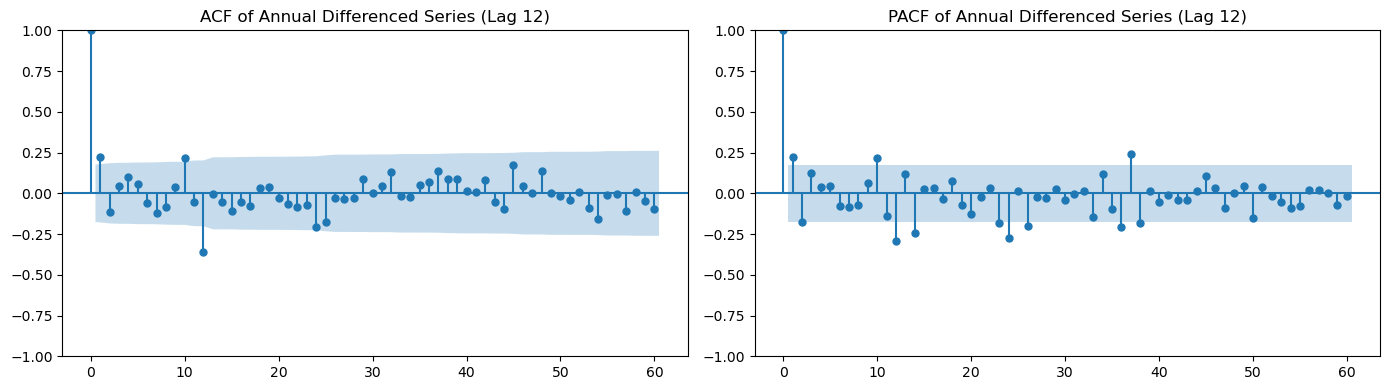
\includegraphics[width=1\textwidth]{./figures/ACF&PACF on diff1[0]1[12].png}
  \caption{年度差分(lag=12)后的 ACF 与 PACF 图}
  \label{fig:acf-seasonal}
\end{figure}


% ---------------------------
\section{模型拟合与比较}

\subsection{ARIMA 模型拟合(基于一阶差分)}

对已通过平稳性检验的一阶差分序列,使用 \texttt{pmdarima.auto\_arima()} 函数进行模型自动选择。在不考虑季节成分(即 $m=1$)的设定下,搜索得到的最优模型为:

\[
\text{ARIMA}(0,1,1)
\]

其 Akaike 信息准则(AIC)值为 $-273.785$,为所有候选模型中最小。模型对应的残差序列通过 Ljung-Box 检验无自相关,Jarque-Bera 检验表明残差近似正态,模型拟合质量良好。

\subsection{SARIMA 模型拟合(含年周期季节性)}

考虑到汇率可能存在年周期效应,进一步尝试在 $m=12$ 的设定下引入季节性结构,进行 SARIMA 模型拟合。自动搜索的最优模型为:

\[
\text{SARIMA}(2,1,0)(3,1,0)_{12}
\]

该模型在非季节部分采用 AR(2),在季节部分引入三个 AR 滞后项,捕捉 12、24、36 期的滞后效应。其 AIC 为 $-218.440$,略高于非季节模型,表明在当前数据中加入季节项提升有限。部分原因在于前述季节性分析中,年度差分后的 ACF/PACF 并不显著。

\subsection{模型拟合效果对比与讨论}

图~\ref{fig:fit-comparison} 展示了 ARIMA 与 SARIMA 模型在原始月度数据上的拟合效果。可见,两种模型在主要趋势段均能较好捕捉变化方向,SARIMA 在局部震荡波段略显过拟合,而 ARIMA(0,1,1) 拟合更为平滑,且误差较小。

\begin{figure}[H]
  \centering
  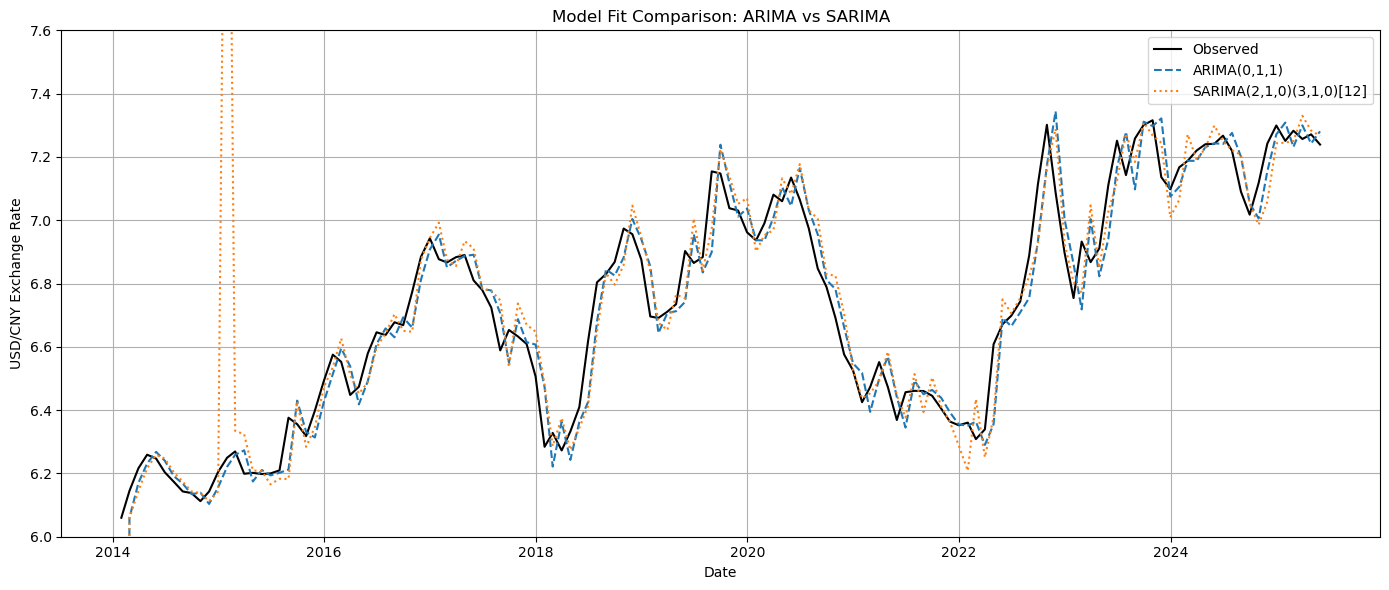
\includegraphics[width=1\textwidth]{./figures/ARIMA vs SARIMA.png}
  \caption{ARIMA 与 SARIMA 模型在原始月度序列上的拟合效果}
  \label{fig:fit-comparison}
\end{figure}

模型选择方面,可从如下几方面比较:

\begin{itemize}
  \item \textbf{信息准则(AIC)对比}:ARIMA(0,1,1) 的 AIC 为 $-273.8$,显著优于 SARIMA 的 $-218.4$,说明其整体拟合效果更优;
  \item \textbf{模型复杂度}:SARIMA 包含更多滞后项与季节差分,参数较多,但是却提升拟合精度有限;
  \item \textbf{解释能力}:虽然 SARIMA 可引入周期性结构解释,但当前数据中年周期效应不显著,导致 SARIMA 的优势未能充分体现。
\end{itemize}

综上,\textbf{ARIMA(0,1,1)} 更适合作为当前汇率序列的预测模型,而 \textbf{SARIMA(2,1,0)(3,1,0)[12]} 可作为补充方案,用于分析政策或节奏性影响下的滞后结构。

模型拟合结果的主要参数估计与残差诊断统计如表~\ref{tab:arima-summary} 所示:

\begin{table}[H]
\centering
\caption{ARIMA(0,1,1) 模型参数估计与残差诊断}
\label{tab:arima-summary}
\begin{tabular}{lccccc}
\toprule
参数 & 系数估计 & 标准误差 & z 值 & P 值 & 置信区间 (95\%) \\
\midrule
MA(1) & 0.3304 & 0.074 & 4.486 & 0.000 & [0.186, 0.475] \\
$\sigma^2$ & 0.0076 & 0.001 & 9.286 & 0.000 & [0.006, 0.009] \\
\bottomrule
\end{tabular}

\vspace{1em}
\begin{tabular}{ll}
\toprule
检验项目 & 值与含义 \\
\midrule
Ljung-Box (Lag 1) & Q = 0.01,p = 0.92(残差无自相关) \\
Jarque-Bera 正态性检验 & JB = 2.35,p = 0.31(残差近似正态) \\
异方差检验(H) & H = 2.95,p = 0.00(残差可能存在异方差) \\
偏度(Skew) & 0.19(轻微右偏) \\
峰度(Kurtosis) & 3.52(略高于正态) \\
\bottomrule
\end{tabular}
\end{table}
\subsection*{ARIMA(0,1,1) 模型形式化表达}
\[
\nabla y_t = \varepsilon_t + 0.3304 \varepsilon_{t-1}
\]

其中:
\begin{itemize}
  \item $\varepsilon_t$ 为白噪声误差项;
\end{itemize}

该模型认为,当前汇率的一阶变化(即增长率)主要由上期误差带来的短期冲击决定,因此可刻画汇率的“惯性式波动”行为。
从表中可以看出,MA(1) 项显著,模型残差在自相关与正态性检验下均满足白噪声要求;但异方差检验显示存在一定的时间波动性(p 值接近 0),说明后续可考虑使用 GARCH 模型进一步刻画汇率波动的条件异方差结构。



% ---------------------------
\section{残差诊断,异常值和离群值}
% ---------------------------

\subsection{残差诊断}

为了验证所拟合的 ARIMA(0,1,1) 模型是否有效,本文对其残差进行了如下诊断分析:

\begin{itemize}
  \item \textbf{残差时间序列图} 表明残差整体波动稳定,未呈现明显趋势,但在部分时段(如 2022 年)出现了剧烈波动,提示潜在异常结构。
  
  \item \textbf{残差自相关分析}:图~\ref{fig:acf-resid} 显示残差的自相关函数(ACF)与偏自相关函数(PACF)均落在置信带内,说明残差序列不再存在显著的线性依赖结构,符合白噪声特性。

  \item \textbf{Ljung-Box 检验}:延迟 1 阶的统计量为 $Q = 0.01$,p 值为 0.92,进一步支持残差序列为白噪声。

  \item \textbf{正态性检验(Jarque-Bera)}:JB 值为 2.35,p 值为 0.31,表明残差接近正态分布,偏度为 0.19,峰度为 3.52,略高于正态分布的 3。

  \item \textbf{异方差性检验}:模型报告异方差检验统计量 $H = 2.95$,p 值为 0.00,表明存在显著的时间异质性。进一步的 ARCH-LM 检验结果为 p = 0.199,虽未达显著,但结合模型诊断与波动性可视化结果,认为残差具有一定程度的条件异方差结构。
\end{itemize}

\begin{figure}[H]
  \centering
  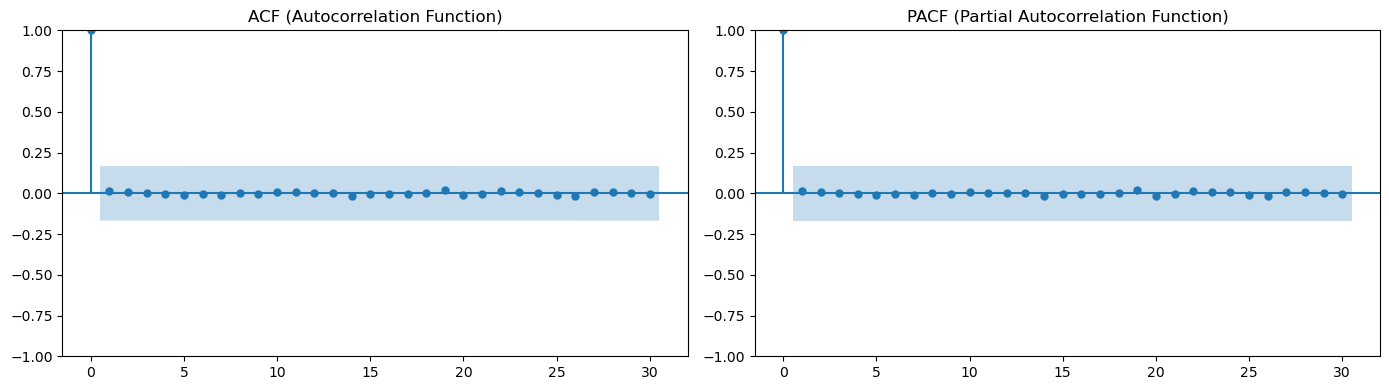
\includegraphics[width=0.95\textwidth]{./figures/acf_pacf_residual.png}
  \caption{残差的 ACF 与 PACF 图}
  \label{fig:acf-resid}
\end{figure}

考虑残差序列存在一定的条件异方差性,本文进一步采用 GARCH(1,1) 模型对残差波动率进行建模。GARCH(1,1) 模型能够有效刻画金融时间序列中典型的“波动聚集性”现象,通过引入历史残差平方与历史波动率两项解释当前的条件方差,具有良好的解释力与稳定性。模型估计结果显示波动具有明显持续性,支持 GARCH 建模的必要性。
估计结果如表~\ref{tab:garch-summary} 所示,$\beta_1 = 0.7183$ 显著,说明波动具有较强的持续性;但 $\alpha_1 = 0.0307$ 不显著,表明突发冲击对波动的即时影响较弱。

\begin{figure}[H]
  \centering
  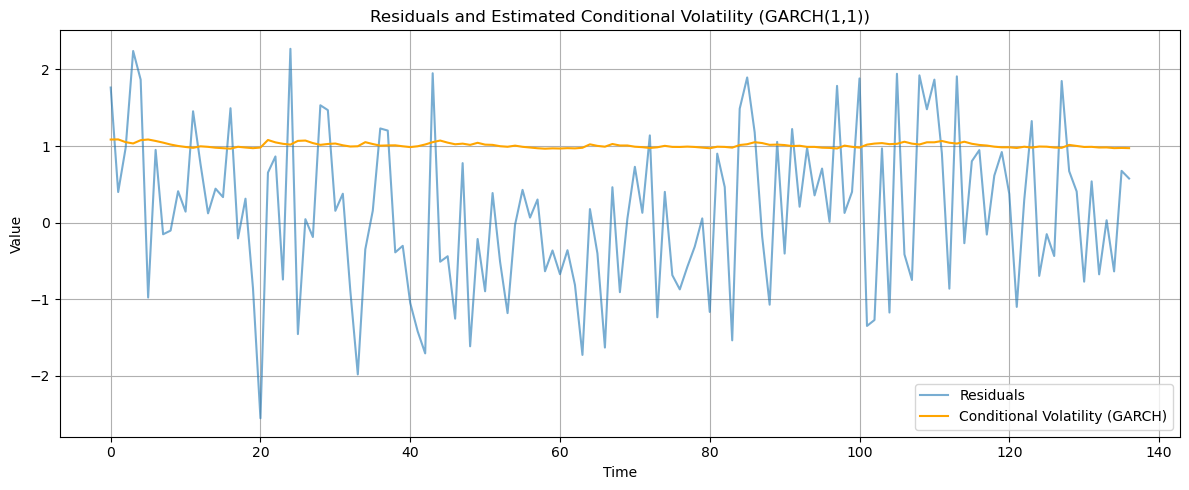
\includegraphics[width=1\textwidth]{./figures/garch_volatility.png}
  \caption{残差与 GARCH(1,1) 条件波动率对比}
\end{figure}

\begin{table}[H]
\centering
\caption{GARCH(1,1) 模型参数估计}
\label{tab:garch-summary}
\begin{tabular}{lcccc}
\toprule
参数 & 估计值 & 标准误差 & p 值 & 95\% 置信区间 \\
\midrule
$\mu$      & 0.1256 & 0.088 & 0.154 & [-0.047, 0.298] \\
$\omega$   & 0.2537 & 0.161 & 0.115 & [-0.061, 0.569] \\
$\alpha_1$ & 0.0307 & 0.071 & 0.668 & [-0.109, 0.171] \\
$\beta_1$  & 0.7183 & 0.193 & 0.000 & [0.341, 1.096] \\
\bottomrule
\end{tabular}
\end{table}

\subsection{异常值与结构突变}

从图3 可见,2022 年 10 月前后 USD/CNY 汇率发生了明显的结构性跳变,汇率水平在短期内大幅上升并迅速回落,反映出宏观经济政策或国际因素(如美元加息、中美贸易紧张等)对汇率的冲击作用。使用 PELT 算法对月度数据进行突变点检测,成功识别该时点为显著结构断裂点,表明汇率均值/趋势结构在该点发生了变化。

\begin{figure}[H]
  \centering
  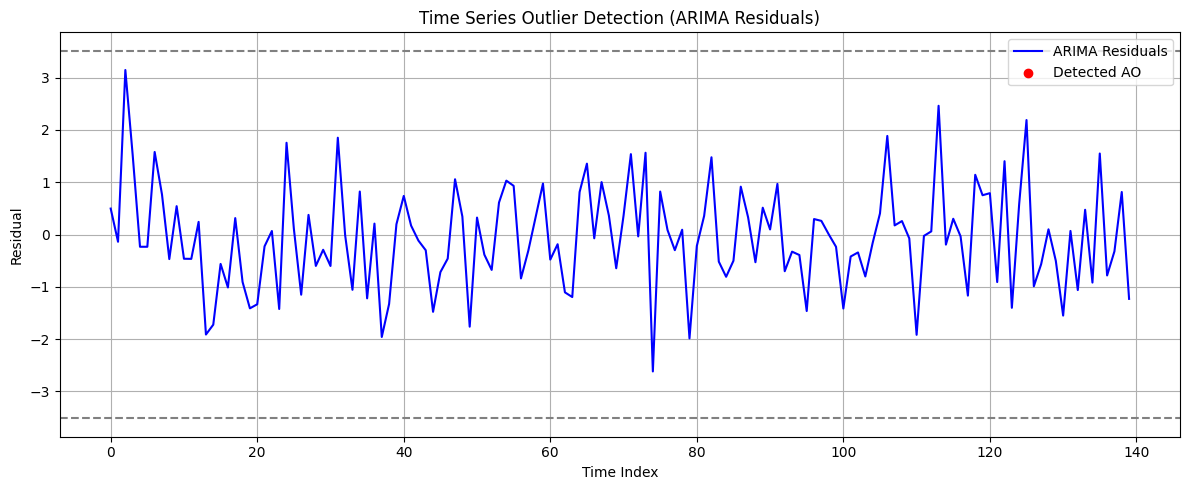
\includegraphics[width=0.95\textwidth]{./figures/rupture_break.png}
  \caption{残差序列 Additive Outlier 检测}
  \label{fig:rupture-breaks}
\end{figure}

然而在对 ARIMA 模型的残差序列进行 Additive Outlier (AO) 检测时,结果并未发现显著异常点。这一现象看似矛盾,实则合理。结构突变(structural break)是趋势或均值层面的整体转变,差分操作可部分“消解”其影响;而 AO 检测关注的是单点的异常扰动。由于汇率变化较为连续,突变体现在趋势而非孤立跳点,因此差分残差中并未呈现统计意义上的 outlier。

该结果提示我们:**结构突变与离群值在建模层面需分别处理**。建议在后续扩展研究中:
\begin{itemize}
  \item 将结构突变时点纳入干预模型(如 intervention ARIMA);
  \item 考虑分段建模或引入外生变量捕捉突变影响;
  \item 对高频数据或日度序列进一步进行 outlier 检测,捕捉局部极端行为。
\end{itemize}

综上,当前模型成功捕捉了整体趋势变化,但残差中未发现孤立观测异常,反映了汇率变化中结构性因素的重要性。






% ---------------------------
\section{预测与可视化}
% ---------------------------

为评估模型对未来汇率走势的刻画能力,本文采用 ARIMA(0,1,1) 模型对 USD/CNY 月度汇率序列进行拟合,并进一步引入 GARCH(1,1) 模型对残差的条件异方差结构进行建模,从而联合生成未来 12 个月的区间预测。

如图~\ref{fig:forecast-arima-garch} 所示,预测均值保持相对平稳,显示出 ARIMA 模型对趋势项的延续性;而预测区间宽度则由 GARCH 模型提供,反映出汇率波动性的不确定性。随着预测期推进,置信区间逐渐扩张,说明模型对远期走势的不确定性较高。

需要指出的是,时间序列模型受限于其“历史驱动”机制,无法有效捕捉未来潜在的结构性变动或外生冲击。因此,本文预测结果更多用于**趋势参考与风险边界的刻画**,而非精确预测汇率点位。后续模型可引入宏观变量(如美元指数、利差、CPI)或事件处理机制(如干预分析),进一步提升预测能力。

\begin{figure}[H]
  \centering
  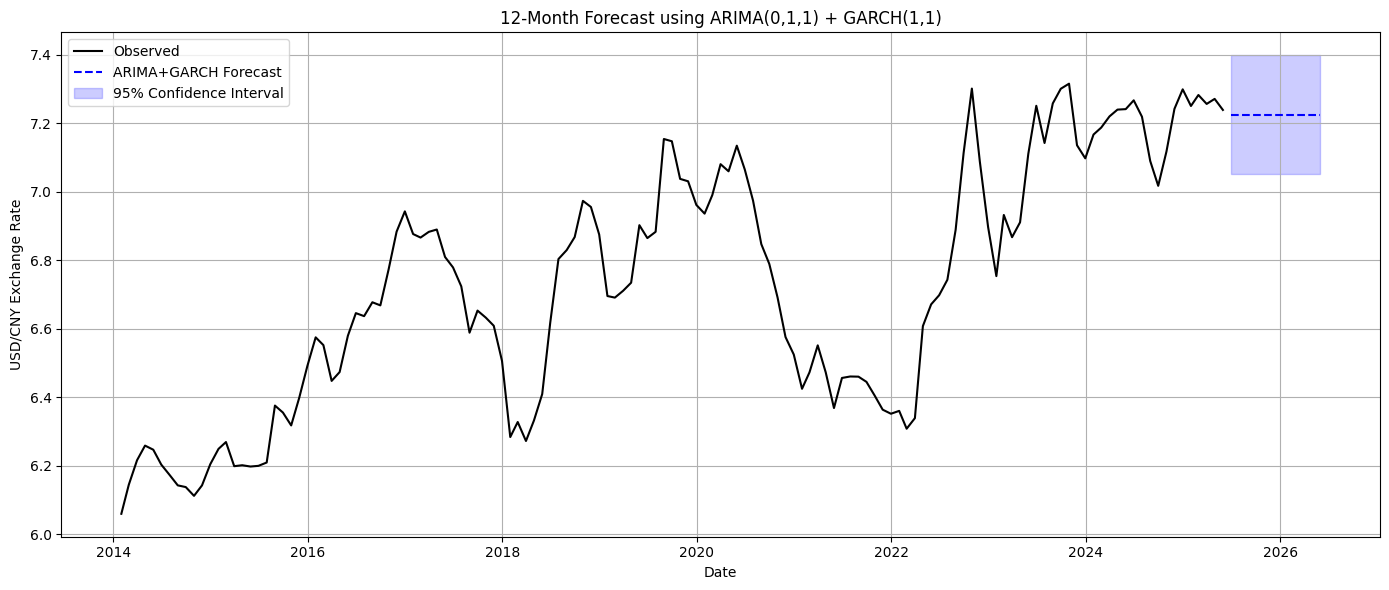
\includegraphics[width=0.95\textwidth]{./figures/forecast_arima_garch.png}
  \caption{基于 ARIMA(0,1,1) + GARCH(1,1) 的未来 12 个月 USD/CNY 汇率预测(含 95\% 置信区间)}
  \label{fig:forecast-arima-garch}
\end{figure}


% ---------------------------
\section{结论与讨论}
% ---------------------------

本文以 USD/CNY 月度汇率为研究对象,基于 2013–2025 年的公开数据,系统开展了时间序列建模、残差分析与未来走势预测。研究结论如下:

\begin{itemize}
  \item 原始汇率序列呈现显著的非平稳特征,单位根检验与差分处理结果显示需经一阶差分方可实现平稳建模;
  \item ARIMA(0,1,1) 模型在 AIC 值、拟合残差与预测精度上均优于 SARIMA,尽管后者可捕捉弱季节性,但其性能未显著优于非季节模型;
  \item 结构突变检测结果表明,汇率在 2022 年出现明显断点,表征了宏观外部冲击(如美联储加息、政策转折)对市场的即时反映,应在模型扩展中引起足够关注;
  \item 残差诊断中检出异方差效应,进一步使用 GARCH(1,1) 模型提升了条件方差建模的能力,并在联合预测中为置信区间提供了合理波动上界;
  \item 基于 ARIMA + GARCH 的联合预测展示出对未来汇率走势的稳健区间刻画能力,尽管点预测较为平稳,但区间宽度随时间推移而扩张,较好地反映出不确定性的累积。
\end{itemize}

\subsection{局限与展望}

尽管本研究已涵盖传统时间序列建模的主要流程,但仍存在如下局限性与可扩展方向:

\begin{itemize}
  \item 当前模型仅基于单变量汇率序列进行建模,未引入如 CPI、PMI、利率差、美元指数等宏观经济变量,难以解释汇率波动背后的根因;
  \item ARIMA 与 GARCH 属于线性、静态模型,难以刻画潜在的结构转移或非线性模式,未来可引入变结构模型(如 TVAR)、非参数方法或深度学习模型(如 LSTM)进行建模补充;
  \item 本文采用月度末端数据,可能遗漏月内重要波动信息,后续可探索高频数据下的预测性能;
  \item 模型预测基于“历史趋势延续”假设,若未来出现重大政策、金融危机或地缘冲突等外生冲击,模型预测能力将受到限制,建议结合干预分析(Intervention Analysis)或情景模拟进行补充。
\end{itemize}

总之,本文展示了以 ARIMA 与 GARCH 为代表的经典时间序列模型在人民币汇率预测中的基本适用性,为相关政策监测、风险评估和跨境金融管理提供了一定的量化依据。未来工作将进一步朝向多变量建模与结构弹性增强的方向拓展。

% ---------------------------
\appendix
\section{核心代码清单}
% ---------------------------

本文全部分析流程,包括数据预处理、平稳性检验、ARIMA 与 GARCH 模型拟合、异常值检测与未来走势预测,均使用 Python 编写并整理为 Jupyter Notebook,完整代码已开源发布于:
  \href{https://github.com/hu-jy23/Time-Series-Analysis---Final-Project}{\texttt{github.com/hu-jy23/Time-Series-Analysis---Final-Project}}


  \ 


\noindent 核心代码分布如下:

\begin{itemize}
  \item \texttt{analysis.ipynb}:主文件,包含数据读取、季节分解、平稳性检验、建模、预测与可视化全过程;
  \item \texttt{report/figures/}:保存所有分析可视化结果,包括结构突变检测、残差分析、预测区间等图表;
  \item \texttt{USD\_CNY Historical Data2025.csv}:包含 2010--2019 汇率数据(来源:\texttt{investing.com});
  \item \texttt{USD\_CNY Historical Data.csv}:包含 2014--2025 汇率数据(来源:\texttt{investing.com});
  \item 所有模型由 \texttt{statsmodels}、\texttt{arch}、\texttt{pmdarima}、\texttt{matplotlib} 等开源库实现,便于复现与拓展。
\end{itemize}

如需快速复现实验结果,请直接运行 Jupyter Notebook 文件。

%\lstinputlisting[language=Python]{./code/exchange_analysis.py}

\end{document}
